\documentclass[fleqn]{beamer}

\usepackage{amsmath}
\usepackage{animate}
\usepackage{amsfonts}
\usepackage[mathscr]{eucal}
\usepackage{subcaption}
\usepackage{wrapfig}
\usepackage{graphicx}

\usepackage{fancyhdr}
\usepackage{pstricks}
\usepackage{pst-func}
\usepackage{pst-plot}
\usepackage[utf8x]{inputenc}
\usepackage[spanish]{babel}


\setbeamertemplate{navigation symbols}{}
\definecolor{UniBlue}{RGB}{83,121,170}
\setbeamercolor{frametitle}{fg=black,bg=white}
\setbeamercolor{title}{fg=black,bg=yellow!85!orange}
%\setbeamercolor{title}{fg=red,bg=yellow!90!blue}
\usetheme{Madrid}

\beamersetuncovermixins{\opaqueness<1>{25}}{\opaqueness<2->{15}}
\begin{document}

\title{Computación Gráfica Avanzada}
\author{Reynaldo Martell}
\date{\today} 

\begin{frame}
\titlepage
\end{frame}

\begin{frame}\frametitle{\rule{0mm}{10mm}\rule{5mm}{0mm} Clases Virtuales - Práctica. }
\begin{enumerate}
	\item La forma de trabajo consistirá en clases virtuales en la plataforma zoom y classroom.
	\item El curso se orientará a clases prácticas en las cuales se harán y subirán videos a un canal de youtube con 14 prácticas en las que se desarrollará el código para que el alumno lo replique y avance a su propio ritmo.
	\item De cada práctica se harán sesiones semanales en las que se aclarén dudas por equipos de la práctica.
	\item Se dejarán ejercicios por cada práctica para que el alumno lo realicé y pueda hacer su reporte.
	\item Las prácticas se subirán a classroom para su revisión.
\end{enumerate}
\end{frame}

\begin{frame}\frametitle{\rule{0mm}{10mm}\rule{5mm}{0mm} Clases Virtuales - Teórica. }
\begin{enumerate}
	\item Las sesiones teóricas se presentarán diapositivas previamenta a la práctica que ayude a complementar la práctica.
	\item El examen se presentará de forma virtual en la plataforma google forms.
\end{enumerate}
\end{frame}

\begin{frame}\frametitle{\rule{0mm}{10mm}\rule{5mm}{0mm} Clases Virtuales - Proyecto. }
\begin{enumerate}
	\item El proyecto final consiste en plantear y desarrollar un videojuego utilizando OpenGL
	\item Se presentará el proyecto en una sesión de zoom y entregará documentación correspondiente.
	\item El proyecto se presentará en equipos y todos son responsables de realizar la entrega y trabajar en el.
\end{enumerate}
\end{frame}

\begin{frame}\frametitle{\rule{0mm}{10mm}\rule{5mm}{0mm} Clases Virtuales - Lineamientos Poryecto. }
\begin{enumerate}
	\item Manejar repositorio remoto git para el código.
	\item Manual de usuario.
	\item Documentación de desarrollo.
	\begin{enumerate}
		\item Objetivo.
		\item Analisis.
		\item Desarrollo.
		\item Resultados.
		\item Trabajo a futuro.
		\item Conclusiones.
	\end{enumerate}
\end{enumerate}
\end{frame}

\begin{frame}\frametitle{\rule{0mm}{10mm}\rule{5mm}{0mm} Computación Gráfica Avanzada. }
Regresando a clases me pueden encontrar en el laboratorio de Proyectos Externos 2, Planta Baja, Edificio U - "Bernardo
Quintana Arrioja“, Facultad de Ingeniería\\
reynaldo.martell@ingenieria.unam.edu
\begin{figure}[H]
	\centering
	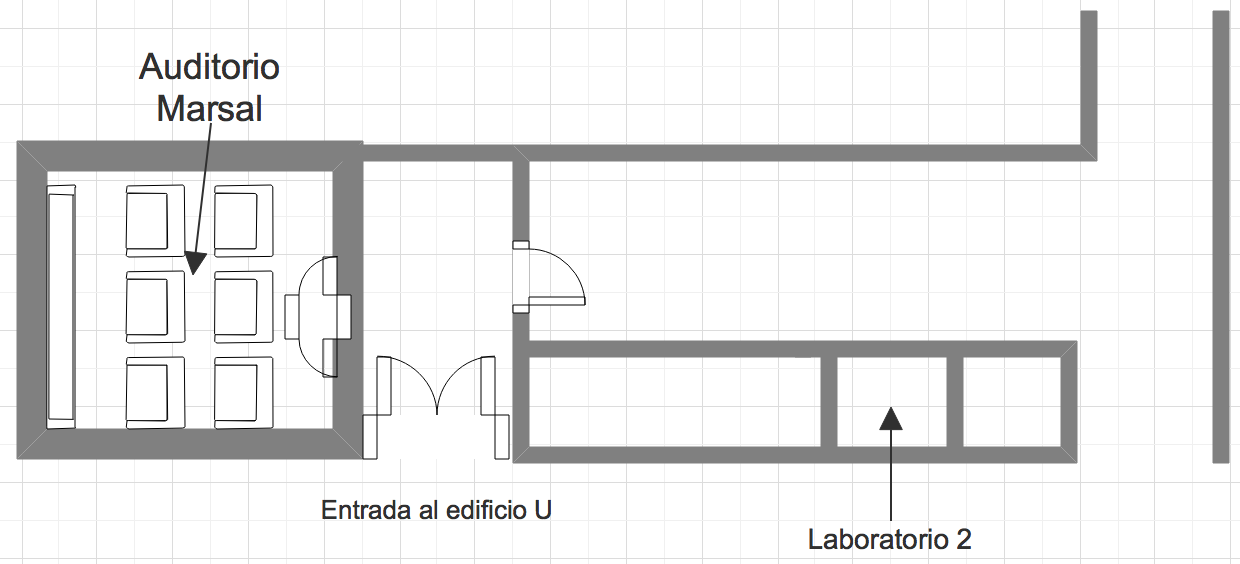
\includegraphics[width=1.0\textwidth]{images/mapa.png}
	\label{mapa}
\end{figure}
\end{frame}

\begin{frame}\frametitle{\rule{0mm}{10mm}\rule{5mm}{0mm} Computación Gráfica Avanzada. }
\begin{enumerate}
	\item Conceptos matemáticos.
	\item Algoritmos de graficación.
	\item Colisiones
	\item C++
	\item OpenGL 4.0
	\item OpenAL audio
	\item Visual studio 2017 (Windows) o Eclipse 2020 (Ubuntu)
\end{enumerate}
\end{frame}

\begin{frame}\frametitle{\rule{0mm}{10mm}\rule{5mm}{0mm} Evaluación. }
\begin{enumerate}
	\item Exámenes 25 \%
	\begin{enumerate}
		\item Parcial 1
		\item Parcial 2
	\end{enumerate}
	\item Proyecto	35 \%
	\item Prácticas 30 \%
	\item Tareas 10 \%
\end{enumerate}
\end{frame}

\begin{frame}\frametitle{\rule{0mm}{10mm}\rule{5mm}{0mm} Evaluación - Consideraciones. }
\begin{enumerate}
	\item No tienen derecho a NP aquellos alumnos que presenten alguno de los
exámenes parciales o el final.
	\item Se exenta del examen final si el promedio es mayor a 6
\end{enumerate}
\end{frame}

\begin{frame}\frametitle{\rule{0mm}{10mm}\rule{5mm}{0mm} Evaluación - Fechas importantes. }
\begin{enumerate}
	\item Primer parcial. 24 de Noviembre.
	\item Segundo parcial. 26 de Enero.
	\item Entrega de proyecto. 2 de Febrero.
	\item Primer examen final. 4 de Febrero.
	\item Segundo examen final. 9 de Febrero.
\end{enumerate}
\end{frame}

\begin{frame}\frametitle{\rule{0mm}{10mm}\rule{5mm}{0mm} Tarea. }
\begin{enumerate}
	\item Tarea inscribirse a classroom: \hfill \break o2gxjgn
	\item Github.
	\begin{enumerate}
		\item Definición.
		\item ¿Qué es un branch?
		\item ¿Qué es un fork?
		\item Utilidad.
		\item Comandos básicos.
		\item Crear cuenta y crear su primer repositorio.
	\end{enumerate}
	\item Instalar las herramientas para el desarrollo.
	\begin{enumerate}
		\item Visual Studio 2017 Windows
		\item Software/Git-2.9.2-64-bit.rar
		\item Software/OpenAL11CoreSDK.rar
	\end{enumerate}
	\item Realizar un Fork del siguiente repositorio.
	\\https://github.com/rmartella/ComputacionGraficaAvanzada
\end{enumerate}
\end{frame}

\end{document}

